\section{Aleatoric limit}
\label{sec:aleatoric}

With a cleaned dataset in hand (§\ref{sec:data_curation}), the next
question is what precision its labels allow.  Solubility is an
experimental quantity, measured in different laboratories with
different instruments and techniques, so every label carries measurement noise; the
disagreement between independent measurements of the same
(solute, solvent, $T$) point is a lower bound on model error that no
predictive method can cross.  This \emph{aleatoric limit} is the
benchmark's ceiling.

The commonly cited $0.6$--$0.8$ log~S figure from
\citet{palmer2014dataquality} has been used to argue that
solubility prediction is ``solved'' once models reach this range.  We
show that (i) this number is the 90--95\textsuperscript{th} percentile
of a heavy-tailed inter-lab distribution rather than the expected
error, and (ii) in expectation inter-lab disagreement is about
$6\times$ smaller.

THE LATTER MAYBE ALSO TO SI:

We build the aleatoric floor in three stages.  §\ref{sec:source}
assembles \emph{independence groups} of DOIs by merging detectable
copies; §\ref{sec:apelblat} fits a temperature-dependent model to each
group for every (solute, solvent) triple it reports; §\ref{sec:epsA}
defines and computes the aleatoric limit $\epsA$ from
Apelblat-interpolated comparisons across those independence groups.

\subsection{Source integrity}
\label{sec:source}

Because a single research group sometimes re-publishes the same
solubility data across multiple papers, treating every DOI as an
independent measurement inflates the apparent sample size and biases
inter-lab statistics toward zero.  We aggregate DOIs into
\emph{independence groups} using two stages of copycat detection,
followed by a reliability ranking against the consensus of other groups.

\paragraph{Stage A — bit-exact.}
DOIs that report an identical four-tuple
$(\mathrm{solute},\mathrm{solvent},\mathrm{round}(T,1),\mathrm{round}(\log_{10} S, 4))$
are unioned deterministically.  No threshold is required: bit-exact
agreement to the fourth decimal across independent DOIs is functionally
impossible as a measurement outcome.  In the cleaned dataset,
\numval{86} such tuples occur, affecting \numval{172} rows across
\numval{46} distinct DOIs; this yields \numval{21} inter-DOI unions.

\paragraph{Stage B' — interpolated gray zone.}
Many copycats publish a re-scaled or slightly relabelled version of the
same data and do \emph{not} satisfy bit-exact equality, so Stage~A
misses them.  After fitting per-group Apelblat / van't-Hoff curves
(§\ref{sec:apelblat}), for every preliminary-group pair sharing a
$(\mathrm{solute},\mathrm{solvent})$ pair we compute the MAE between
their fitted curves evaluated on a uniform 1~K reference grid in the
intersection of their fit ranges (overlap $\geq 5$~K required).  Pairs
whose weighted MAE across all shared (solute, solvent) pairs falls below
$\theta_{B'} = 0.01$ log~S are unioned.  This yields \numval{55}
additional unions, producing \numval{1\,415} final independence groups
(down from \numval{1\,493} DOIs): a size histogram of \numval{1\,348}
singletons, \numval{57} pairs, \numval{8} triples, \numval{2}
quadruples.

Figure~\ref{fig:source_integrity}(a) shows the distribution of these
interpolated pair-MAEs.  The $\theta_{B'} = 0.01$ cut sits in a sparse
region of the distribution: only \numval{55} of \numval{373} tested
preliminary-group pairs fall below it, while the bulk of the mass lies
well above at \numval{0.02}--\numval{1} log~S (genuine inter-lab
disagreement).

\paragraph{Why 0.01?}
The threshold $\theta_{B'}$ controls a trade-off: too small a value
leaves obvious copies in the multi-source pool where they deflate
$\epsA$ artificially; too large a value merges genuinely agreeing labs,
shrinks the multi-source pool, and inflates $\epsA$ among the smaller
remaining pairs.  Figure~\ref{fig:threshold_sweep} shows the empirical
curve.  Below $\theta = 0.007$ very few additional unions are made: the
multi-source pair count barely decreases (from \numval{566} at $\theta
= 0$ to \numval{521} at $\theta = 0.007$, 8\,\% loss) and $\epsA$ rises
only 8\,\% (from \numval{0.091} to \numval{0.098}).  Between $\theta =
0.010$ and $\theta = 0.020$ there is a cliff in the pair count: from
\numval{484} pairs to \numval{378} pairs, a loss of \numval{106} pairs
over a 0.01-log-S interval (more than the entire loss for $\theta \in
[0, 0.01]$).  At the same time $\epsA$ jumps by 21\,\%, from
\numval{0.105} to \numval{0.127}.  Beyond $\theta = 0.05$ the
multi-source pool has more than halved.  We therefore adopt $\theta =
0.01$ as the conservative upper edge of the ``copycats-only'' region:
it merges the detectable copies while preserving the largest possible
multi-source pool for downstream analysis.

\paragraph{Stage C' — interpolated reliability.}
For each final group, we evaluate its fitted curves at a uniform 1~K
grid on the intersection of all groups' fit ranges for every
(solute, solvent) pair where the group co-appears.  At each grid point
the \emph{consensus} is the mean of the \emph{other} groups' fitted
values; the group's local deviation is the absolute difference between
its own value and the consensus.  Averaged across all grid points the
group participates in, this produces a single reliability score per
group.  Groups scoring $\leq 0.2$ log~S form the \emph{Hall of Fame};
groups scoring $\geq 0.6$ join the \emph{Hall of Shame}
(Figure~\ref{fig:source_integrity}(b)).  Of \numval{1\,415} final
groups, \numval{399} have enough cross-group overlap to be tested;
\numval{316} land in the Hall of Fame and \numval{27} in the Hall of
Shame.

\begin{figure}[t]
  \centering
  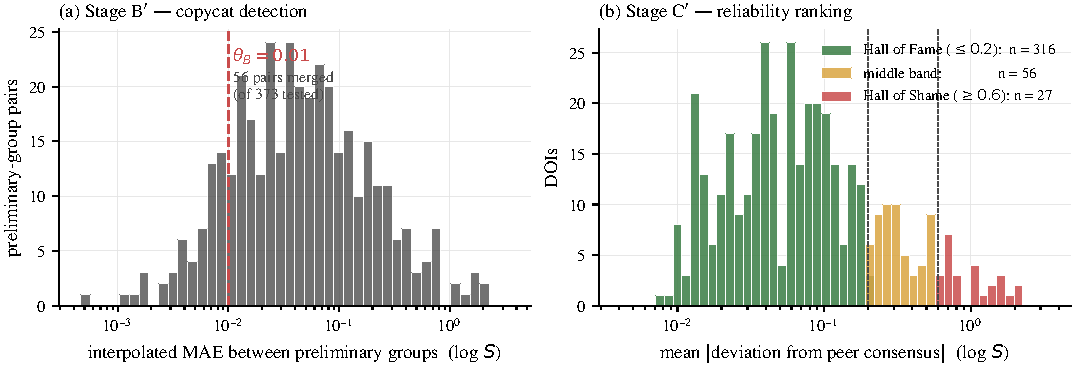
\includegraphics[width=\linewidth]{figures/fig_source_integrity.pdf}
  \caption{\textbf{(a) Stage B$'$ copycat detection.}  Distribution of
    interpolated pair-MAE between preliminary-group pairs sharing at
    least one (solute, solvent) pair.  Dashed line = $\theta_{B'} =
    0.01$ log~S cut.  \textbf{(b) Stage C$'$ reliability ranking.}
    Distribution of per-group mean absolute deviation from peer
    consensus on Apelblat-interpolated curves.  Hall of Fame
    ($\leq 0.2$), middle band, and Hall of Shame ($\geq 0.6$) are
    coloured; dashed vertical lines are the cut-offs.}
  \label{fig:source_integrity}
\end{figure}

\begin{figure}[t]
  \centering
  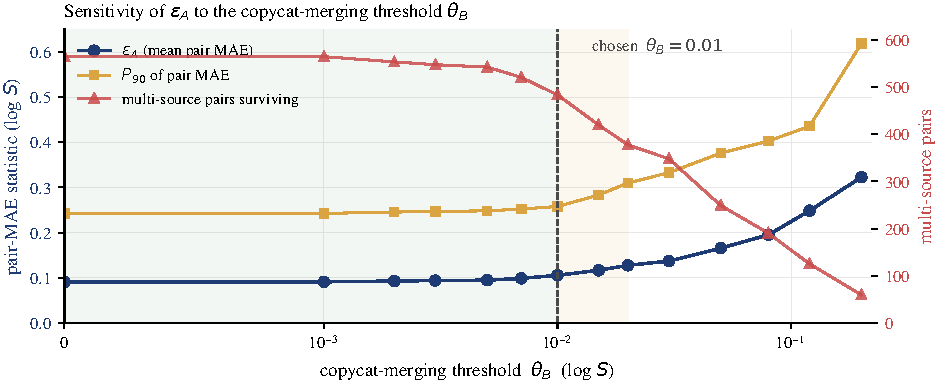
\includegraphics[width=0.9\linewidth]{figures/fig_threshold_sweep.pdf}
  \caption{Sensitivity of $\epsA$ and the multi-source pair count to the
    copycat-merging threshold $\theta_B$.  The chosen value $\theta_B =
    0.01$ (dashed line) sits at the upper edge of the shaded ``safe''
    region, where each merged pair is a genuine copy.  The shaded
    ``cliff'' region $[0.01, 0.02]$ loses $\numval{106}$ multi-source
    pairs --- more than the entire loss incurred between $0$ and
    $0.01$.}
  \label{fig:threshold_sweep}
\end{figure}

\subsection{Thermodynamic curve fits}
\label{sec:apelblat}

To compare laboratories that do not share exact measurement
temperatures, we fit a smooth thermodynamic model to every
$(\mathrm{solute},\mathrm{solvent},\mathrm{group})$ triple with
$\geq 3$ temperature points:

\begin{equation}
  \log_{10} S \;=\; A \;+\; \frac{B}{T} \;+\; C\,\ln T \qquad (\text{Apelblat}),
  \label{eq:apelblat}
\end{equation}

and a reduced form to triples with exactly two temperature points:

\begin{equation}
  \log_{10} S \;=\; A \;+\; \frac{B}{T} \qquad (\text{van't~Hoff}).
  \label{eq:vant}
\end{equation}

Triples with a single temperature point (\numval{507}, $\sim 4.5$\,\%)
cannot be fitted and are excluded from aleatoric interpolation.  Fits
with $R^2 < 0.80$ or RMSE $> 0.30$ log~S (\numval{16}) are flagged as
low-quality and also excluded.  The remaining \numval{11\,063} fits
cover $\geq 95$\,\% of the cleaned data.

Figure~\ref{fig:apelblat}(a) shows the fit-quality distribution: median
$R^2 = 0.9993$, \numval{99.3\,\%} of fits reach $R^2 \geq 0.95$,
\numval{94.9\,\%} reach $R^2 \geq 0.99$.  Thermodynamic monotonicity is
similarly strong: \numval{98.5\,\%} of triples are strictly
monotone-increasing in temperature and only \numval{1} triple shows a
single-step drop exceeding $1$~log~S.
Figure~\ref{fig:apelblat}(b) shows the distribution of per-fit
temperature coverage $\Delta T = T_{\max} - T_{\min}$.  The median
fit spans \numval{30}~K and only a small minority of fits cover less
than the 5~K minimum required for cross-group interpolation
(§\ref{sec:epsA}), confirming that the Apelblat framework supports
aleatoric analysis on the majority of the multi-source pool without
extrapolation.

\begin{figure}[t]
  \centering
  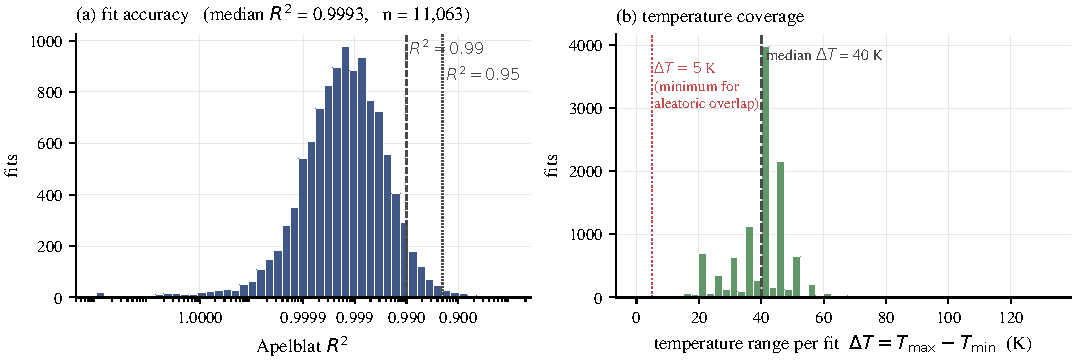
\includegraphics[width=\linewidth]{figures/fig_apelblat_quality.pdf}
  \caption{Apelblat fit quality.  \textbf{(a)}~$R^2$ distribution on a
    reversed log scale ($1 - R^2$ axis).  Most fits have
    $R^2 > 0.99$.  \textbf{(b)}~Temperature coverage $\Delta T$ per
    fit.  Most fits cover more than the 5~K minimum needed for aleatoric
    interpolation; the median fit spans \numval{30}~K.}
  \label{fig:apelblat}
\end{figure}

\subsection{Aleatoric limit}
\label{sec:epsA}

With independence groups and per-group curves established, the
aleatoric limit is a single pair-level statistic on this structure.

\paragraph{Mathematical framework.}
For an $(\mathrm{solute},\mathrm{solvent})$ pair at temperature $T$, the
true solubility $\log_{10} S^{*}(T)$ is unknown.  Independence group $i$
observes $y_i(T) = \log_{10} S^{*}(T) + \varepsilon_i(T)$, where
$\varepsilon_i$ is measurement noise plus any systematic lab effect.
Given fitted curves $f_i(T)$ and $f_j(T)$ for groups $i$ and $j$ on a
reference grid $\mathcal{T}_{ij} = [T^{\min}_{ij}, \ldots, T^{\max}_{ij}]$
at $\Delta T = 1$~K, the interpolated inter-group disagreement at cell
$T$ is

\begin{equation}
  \varepsilon_{ij}(T) \;=\; \bigl|\,f_i(T) - f_j(T)\,\bigr|,
  \label{eq:eps_ij}
\end{equation}

and the \emph{group-pair} MAE is $\mathrm{MAE}_{ij} =
\mathrm{mean}_{T \in \mathcal{T}_{ij}}\,\varepsilon_{ij}(T)$.  Per
(solute, solvent) pair $p$ with independence groups $\mathcal{G}_p$, the
\emph{pair} MAE averages over all within-pair group pairs:

\begin{equation}
  \mathrm{MAE}_p \;=\; \frac{1}{\binom{|\mathcal{G}_p|}{2}}
  \sum_{i<j \in \mathcal{G}_p} \mathrm{MAE}_{ij}.
  \label{eq:mae_pair}
\end{equation}

The aleatoric limit is the \emph{mean} pair MAE across the multi-source
pool $\mathcal{P}$:

\begin{equation}
  \boxed{\;\epsA \;=\; \frac{1}{|\mathcal{P}|}
         \sum_{p \in \mathcal{P}} \mathrm{MAE}_p.\;}
  \label{eq:epsA}
\end{equation}

Two aspects warrant emphasis.  First, $\epsA$ is an \emph{error in
expectation} over pairs and group-pair comparisons, not a summary of
the heavy tail (reported separately below).  Second, we evaluate
\emph{every} cell via the fitted curve (never a measured value) so the
comparison is uniform in character and not biased toward pairs that
happen to share exact measured temperatures.

\paragraph{Primary vs inclusive.}
The Hall-of-Shame groups identified in §\ref{sec:source} consist
overwhelmingly of systematic publication errors (unit swaps, density
errors, silent transcription mistakes) rather than random measurement
noise.  They are excluded from tier consensus labels
(§\ref{sec:tiers}).  For the
aleatoric limit, we report both variants: a \emph{primary} value that
excludes HoS groups (the floor relevant to benchmark performance,
because tier labels use the same pool), and an \emph{inclusive} value
that retains them (useful when comparing against the broader
literature).

\begin{table}[h]
\centering\small
\caption{Primary and inclusive $\epsA$.  95\,\% confidence intervals are
from 5\,000 bootstrap resamples over the multi-source pair pool.}
\label{tab:epsA}
\begin{tabular}{@{}lccccccc@{}}
\toprule
             & $n$ pairs & mean = $\epsA$ & 95\,\% CI       & median & $P_{90}$ & $P_{95}$ & RMSE \\
\midrule
\textbf{Primary} (HoS-excluded)
             & 481       & \textbf{0.106} & [0.093, 0.120] & 0.046  & 0.258    & 0.385    & 0.182 \\
Inclusive    & 511       & 0.158          & [0.132, 0.186] & 0.050  & 0.385    & 0.627    & 0.356 \\
\bottomrule
\end{tabular}
\end{table}

The 95\,\% CI on $\epsA$ (primary) excludes zero by about 7~standard
errors --- the floor is precisely characterised.

\paragraph{Distribution shape.}
Figure~\ref{fig:aleatoric_main} shows the per-pair MAE distribution
together with a gamma fit to the atom-level $|\Delta|$ distribution.
The gamma shape parameter $\alpha = 0.68$ confirms a sub-exponential
(heavy) right tail, which is why the mean (\numval{0.106}) lies well
above the median (\numval{0.046}).  Panel (b) plots the survival
function: 5\,\% of pairs disagree by more than \numval{0.39} log~S, and
the 99\textsuperscript{th}-percentile pair disagrees by more than
$1$~log~S.

\begin{figure}[t]
  \centering
  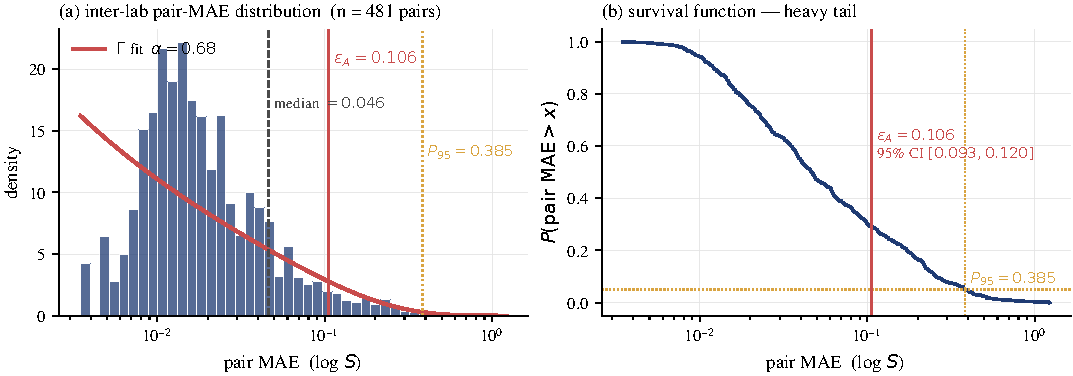
\includegraphics[width=\linewidth]{figures/fig_aleatoric_main.pdf}
  \caption{Primary aleatoric distribution (HoS-excluded).
    \textbf{(a)}~Density of per-pair MAE on log-$x$ axis with a gamma
    fit overlay ($\alpha = 0.68$).  \textbf{(b)}~Survival function
    $P(\mathrm{MAE} > x)$.  Heavy right tail: $P_{95} = 0.39$ log~S.}
  \label{fig:aleatoric_main}
\end{figure}

\paragraph{Per-solvent heterogeneity.}
$\epsA$ is not uniform across solvents (Figure~\ref{fig:per_solvent}).
DMF has the tightest inter-lab agreement at \numval{0.029} log~S across
10 pairs.  Water --- often assumed to be well-characterised because of
the large volume of aqueous data --- has the \emph{highest} mean among
common solvents (\numval{0.110} log~S across \numval{65} pairs), driven
by a thicker tail rather than a higher typical disagreement (its median
is only \numval{0.061}).  This per-solvent heterogeneity motivates the per-solvent evaluation
metric proposed in §\ref{sec:metric_suite} (PS-RMSE): a single global
$\epsA$ under-characterises measurement quality in difficult solvents
and over-characterises it in well-behaved ones.

\begin{figure}[t]
  \centering
  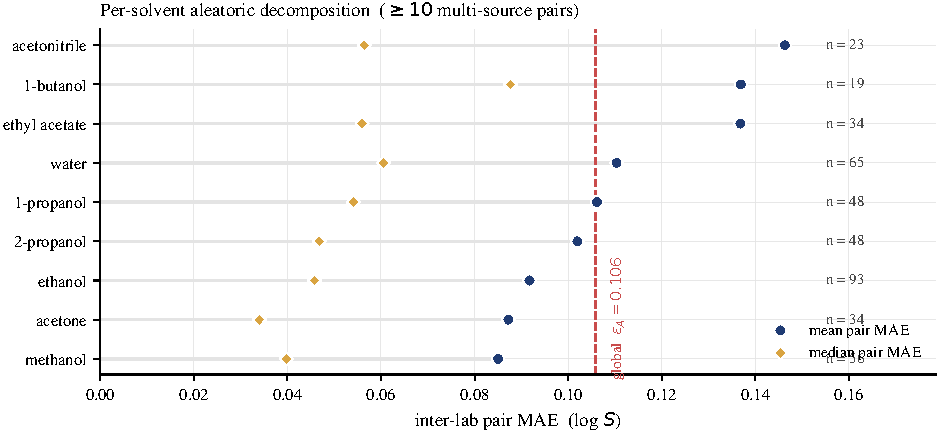
\includegraphics[width=0.95\linewidth]{figures/fig_per_solvent.pdf}
  \caption{Per-solvent aleatoric decomposition (primary, HoS-excluded,
    solvents with $\geq 10$ multi-source pairs).  Lollipops are mean
    pair MAE; diamonds are median; $n$ is the multi-source pair count.
    Dashed vertical line is the global $\epsA = 0.106$.}
  \label{fig:per_solvent}
\end{figure}

\paragraph{Reconciliation with Palmer \& Mitchell (2014).}
The \numval{0.6--0.8} log~S figure cited in the aqueous-solubility
literature is not wrong --- it is simply a different summary statistic
on the same underlying distribution.  Figure~\ref{fig:palmer} overlays
our full inclusive atom-level $|\Delta|$ distribution with the Palmer
band (shaded).  Their number coincides with \emph{our} $P_{90}$--$P_{95}$
at \numval{0.39}--\numval{0.63} log~S and with our RMSE (\numval{0.36}),
but not with the mean (\numval{0.16}) or median (\numval{0.05}).  A
practitioner who quotes the \emph{expected} inter-lab error --- the
number models compete against in expectation --- should quote
$\epsA \approx \numval{0.11}$ log~S; a practitioner who quotes the
95\textsuperscript{th}-percentile worst case --- the noise a model
faces on its hardest test point --- can legitimately still quote
\numval{0.6}.

\begin{figure}[t]
  \centering
  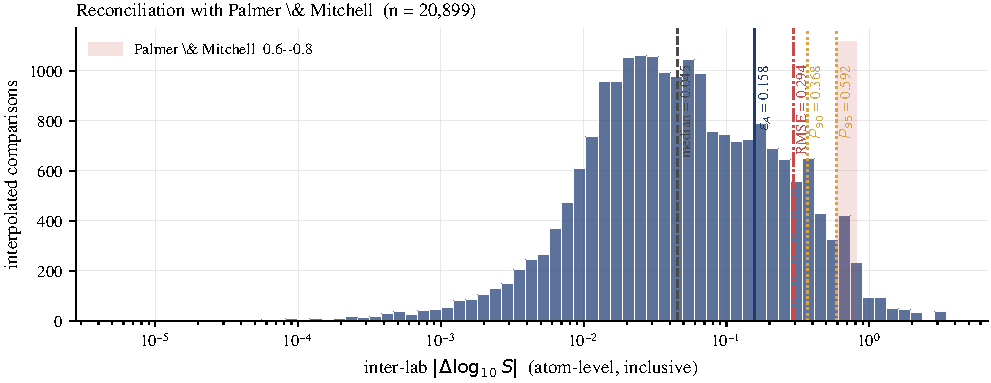
\includegraphics[width=0.9\linewidth]{figures/fig_palmer.pdf}
  \caption{Reconciliation with \citet{palmer2014dataquality}.  The
    inclusive atom-level $|\Delta \log_{10} S|$ distribution
    ($n = 20\,899$ interpolated comparisons) is plotted on a log-$x$
    axis; vertical lines are our summary statistics.  The shaded band
    is Palmer \& Mitchell's quoted 0.6--0.8 log~S aqueous range, which
    coincides with our $P_{90}$--$P_{95}$ and RMSE, not with the
    expected error.}
  \label{fig:palmer}
\end{figure}

\paragraph{Cross-database validation.}
Our $\epsA$ characterises consistency \emph{within} \textsc{BigSolDB}
after copycat correction and Hall-of-Shame exclusion.  A natural
question is whether this floor extends across databases compiled from
different source selections and unit conventions.

\todo{Cross-database validation not yet computed.  Plan: match aqueous
compounds common to \textsc{BigSolDB} and \textsc{AqSolDB}
\citep{sorkun2019aqsoldb} under our Option-D canonicalization, report
matched-set size, RMSE, MAE and systematic bias, and compare to the
intra-\textsc{BigSolDB}{} $\epsA$ reported above.  Expect the
cross-database disagreement to be substantially larger than $\epsA$
owing to differences in unit convention, source selection and
temperature handling across the two databases.}

Independently of the exact cross-database number, the intra-database
floor reported above is the ceiling relevant to our \scthree{}
benchmark, because \scthree{} is constructed entirely from
\textsc{BigSolDB}.
